\chapter{Onderzoek}
\label{ch:onderzoek}

Het kiezen voor een bepaald \gls{compressie-algoritme} is zeer \gls{use-case} gebonden. Zeker binnen \gls{videocompressie} en \gls{afbeeldingscompressie} is dit het geval. Ligt de focus op een zo klein mogelijke bestandsgrootte of juist op het behouden van zo veel mogelijk kwaliteit binnen een bepaalde omgeving? Wordt er voor een \gls{lossless} of \gls{lossy} \gls{compressie-algoritme} gekozen?

Zoals besproken in hoofdstuk \ref{ch:kwaliteit} zijn er zowel objectieve als subjectieve onderzoeken die kunnen gevoerd worden om een gepast \gls{compressie-algoritme} te bepalen. In dit hoofdstuk wordt een subjectief onderzoek uitgevoerd voor het bepalen van een geschikt \gls{afbeeldingsformaat} binnen een bepaalde \gls{use-case}. De gebruikte \gls{afbeeldingsevaluatietool} is ontwikkeld voor deze bachelorproef en is \gls{open-source} en gratis in gebruik. De code is te vinden op de \gls{github} repository van deze bachelorproef\urlcite{githubbachelorproef}. Dit maakt het heel eenvoudig dit onderzoek te reproduceren of een gelijkaardig onderzoek uit te voeren met andere \glspl{afbeeldingsformaat} en/of voor een andere \gls{use-case}.

%TODO: onderzoek

\section{Waarom een subjectief onderzoek}
\label{sec:onderzoek-waarom-subjectief}

Zoals besproken in hoofdstuk \ref{ch:kwaliteit} is een subjectief onderzoek aangeraden binnen tal van \glspl{use-case}. Zeker binnen visuele \gls{datacompressie} kan dit de aangeraden manier van werken zijn aangezien de kwaliteit van de afbeeldingen een grote invloed heeft op de gebruikerservaring. 

Een objectief onderzoek dat bijvoorbeeld werkt aan de hand van het vergelijken van een afbeelding voor en na compressie kan een vals positief of negatief beeld geven over een bepaald \gls{afbeeldingsformaat}.

\section{Use case}
\label{sec:onderzoek-use-case}

De \gls{raw} bestanden gebruikt binnen dit onderzoek zijn aangeleverd door Mayté Bogaert, van MaytéB fotografie. Aangezien zij ook aan het plannen is een online portfolio te bouwen vroeg ze zich af in welk \gls{afbeeldingsformaat} en met welke \gls{render} instellingen ze de afbeelding het best online zet. Deze vraag is dan ook de \gls{use-case} van dit onderzoek.

Voor deze \gls{use-case} speelt de gebruikerservaring een zeer belangrijke rol. Als fotografe zijn afbeeldingen je product en moeten potentiële klanten deze dus positief ervaren wanneer ze op je portfolio terecht komen.

Langs de andere kant gaat het om een online website en moet er dus rekening gehouden worden met \gls{hosting} kosten, wachttijden en \gls{bandbreedte} gebruik. Als de website te lang duurt om te laden of alle mobiele data van een potentiële klant opgebruikt is dat geen goede reclame.

Er wordt dus een \gls{afbeeldingsformaat} gezocht met (zeer) goede beoordelingen uit het onderzoek dat de kleinste bestandsgrootte heeft.

\section{Afbeeldingsevaluatietool}
\label{sec:onderzoek-evaluatietool}

De gebruikte \gls{afbeeldingsevaluatietool} voor het voeren van dit onderzoek is een voor deze bachelorproef ontwikkelde \gls{afbeeldingsevaluatietool}. De code is te vinden op de \gls{github} repository van deze bachelorproef\urlcite{githubbachelorproef}. 

Deze tool is geschreven in \gls{php} met een achterliggende \gls{sql} databank. Dit maakt het mogelijk de tool eenvoudig lokaal te runnen door het gebruik van webserver omgevingen als \gls{xampp} of online te plaatsen op de meeste \gls{hosting} platformen.

De \gls{afbeeldingsevaluatietool} maakt gebruik van een 50\% grijze achtergrond doorheen de ondervraging. Dit is de aangeraden kleur om geen impact te hebben op de perceptie van de kleuren binnen de afbeelding. Het inzoomen gebeurt aan de hand van pure \gls{js} waardoor geen manipulaties aan de afbeelding gebeuren en deze worden weergegeven zoals ze opgeslagen zijn. 

\subsection{Opzetten van de afbeeldingsevaluatietool}
\label{sec:onderzoek-evaluatietool-setup}

Een identiek onderzoek maar met andere afbeeldingen kan gevoerd worden zonder code aanpassingen te moeten uitvoeren wat de reproduceerbaarheid van dit onderzoek hoog houd. 

Plaats hiervoor de bronbestanden op de webserver en voorzien een database via localhost genaamd 'bachelorproef'. De gebruiker root met wachtwoord root moet toegang hebben tot deze database. Plaats de te evalueren afbeeldingen onder de map 'evaluatiereeks' en/of 'testreeks' te vinden in de map 'evaluatie\_afbeeldingen'. Surf naar '/setup.php' en wacht tot er 'done' op het scherm verschijnt. Het onderzoek is nu klaar om te starten en kan via de hoofdfolder gestart worden ('/index.php').

Let wel op dat het testtoestel over de nodige browsers beschikt die de te evalueren \glspl{afbeeldingsformaat} ondersteund en dat \gls{js} ondersteuning aanstaat. Websites als caniuse.com zijn ideaal om na te gaan welke browser en toestellen welke \glspl{afbeeldingsformaat} ondersteund.

Voor het opzetten van de \gls{afbeeldingsevaluatietool} met andere instellingen zoals meer ondervraagde kenmerken of \glspl{afbeeldingsformaat} zijn echter wel aanpassingen aan de code vereist. 

\subsubsection{Afbeeldingsevaluatietool instellingen en uitbreidingen}
\label{sec:onderzoek-evaluatietool-setup-database}

De database instellingen en \gls{sql} query's zijn bewaard onder 'db\_actions.php' te vinden onder de map 'db'. Bovenaan deze file kunnen de servernaam en databasenaam aangepast worden alsook de gebruikersnaam en het wachtwoord.

Mochten er extra bij te houden variabelen gewenst zijn kunnen deze toegevoegd worden in de functie 'create\_tables()' onder 'db\_actions.php'. Deze acties worden opgeroepen vanaf 'onderzoek.php', bijkomende input velden en logica kunnen hier dan ook voorzien worden.

De tekst op het eerste scherm is terug te vinden in 'index.php'. De verwijzing naar het filmpje is terug te vinden in 'introductie.php' en kan vervangen worden door een andere \gls{yt} link of een lokaal bestand.

De tool is voorzien van \gls{bootstrap}, \gls{jquery} en \gls{drift}, een \gls{open-source} \gls{js} \gls{plug-in} voor het inzoomen op afbeeldingen. Er is commentaar voorzien in de code waar nodig en functienamen zijn steeds verklarend. Aanpassingen zouden dus mogelijk moeten zijn zonder veel tijd of werk.

\subsection{Verloop  van de afbeeldingsevaluatietool}
\label{sec:onderzoek-evaluatietool-verloop}

De \gls{afbeeldingsevaluatietool} is alomvattend voor het verzamelen van de gegevens omtrent dit onderzoek. Dit wil zeggen dat in de \gls{afbeeldingsevaluatietool} zelf beschreven wordt hoe de deze dient gebruikt te worden en welke gegevens van de deelnemer bewaart worden. De \gls{afbeeldingsevaluatietool} slaat ook alle input van de gebruiker automatisch op in de achterliggende \gls{sql} databank waardoor er geen manueel werk meer nodig is.

Enkele screenshots van de \gls{afbeeldingsevaluatietool} zijn raadpleegbaar in deel \ref{sec:bijlages-screenshot-afbeeldingsevaluatietool}.

\subsection{Verloop  van de afbeeldingsevaluatietool: Introductie}
\label{sec:onderzoek-evaluatietool-verloop-intro}

De deelnemer van het onderzoek wordt gegroet met een scherm dat mededeelt waarover het onderzoek gaat, welke gegevens van de deelnemer gevraagd en bewaard zullen blijven en de geschatte duur van het onderzoek, zijnde een half uur tot drie kwartier. Een screenshot is voorzien in figuur \ref{fig:bijlages-screenshot-afbeeldingsevaluatietool-welkom}.

Als de deelnemer akkoord gaat met de gegevensverwerking wordt deze doorgebracht naar een volgende pagina met een video\urlcite{introductievideo} van 4 minuten op. Hierin worden de geëvalueerde onderdelen uitgelegd aan de hand van enkele extreme voorbeelden. Ook de \gls{use-case} en gegevensverwerking worden nogmaals uitgelegd. Een screenshot is voorzien in figuur \ref{fig:bijlages-screenshot-afbeeldingsevaluatietool-video}.

\subsection{Verloop  van de afbeeldingsevaluatietool: Informatie over deelnemer}
\label{sec:onderzoek-evaluatietool-verloop-info-participant}

Er worden enkele gegevens van de deelnemer gevraagd en opgeslagen zijnde: 

\begin{itemize}
	\item Geslacht (man, vrouw, overige)
	\item Leeftijd
	\item Of de deelnemer expertise heeft binnen het 
	onderzoeksdomein
	\item Of de gebruiker kleurenblind is
	\item Of de gebruiker slechtziend is
\end{itemize}

Het geslacht wordt bijgehouden om na te gaan om na te gaan of het mikpunt van 50/50 verhouding tussen man en vrouw bereikt is.

Een deelnemer wordt beschouwd als expertise hebbende wanneer deze een gegronde kennis heeft van \gls{afbeeldingscompressie} en \glspl{afbeeldingsformaat}, het verschil kent tussen \gls{lossless} en \gls{lossy} \glspl{compressie-algoritme} alsook artifacten zoals blokartifcaten kan herkennen in afbeeldingen.

Kleurenblindheid is een veelvoorkomend probleem bij mannen. Gemiddeld één op twaalf mannen heeft kleurenblindheid terwijl bij vrouwen dat gemiddelde onder de één op 250 ligt volgens \citetitle{porcella2008} (\cite{porcella2008}). Deze variabele wordt samen met slechtziendheid bijgehouden om na te gaan of dit een impact heeft op de perceptie van de afbeeldingen.

Een screenshot van dit scherm is voorzien in figuur \ref{fig:bijlages-screenshot-afbeeldingsevaluatietool-over-u}.

\subsection{Verloop  van de afbeeldingsevaluatietool: beoordeling}
\label{sec:onderzoek-evaluatietool-verloop-beoordeling}

Uiteindelijk krijgt de deelnemer voor elke afbeelding een evaluatiescherm te zien. Een screenshot van dit scherm is voorzien in figuur \ref{fig:bijlages-screenshot-afbeeldingsevaluatietool-evalutie}.

De volgorde van de afbeeldingen is voor elke deelnemer random bepaald. Indien er een testreeks voorzien is worden eerst de afbeeldingen uit deze testreeks aan de deelnemer getoond.

Op dit evaluatiescherm is aan de hand van \gls{drift} de mogelijkheid voorzien op de rechterhelft van het scherm een ingezoomde variant van de afbeelding op de linkerhelft te bekijken. Deze zoom is 5x en wordt bekomen door een pure \gls{js} oplossing. Dit wilt zeggen dat het originele bestand getoond wordt en er dus geen kwaliteitsverlies mogelijk is door deze \gls{plug-in}.

De deelnemer dient de afbeelding te beoordelen op de volgende drie kenmerken met een getal van één tot vijf:

\begin{itemize}
	\item Scherpte
	\item Kleuren en contrast
	\item Algemene indruk
\end{itemize}

\subsubsection{Kenmerk: scherpte}
\label{sec:onderzoek-evaluatietool-verloop-beoordeling-scherpte}

Een afbeelding wordt beschouwd als scherp wanneer de lijnen vloeiend worden weergegeven en er veel detail aanwezig is. Een fragment uit de introductievideo van de \gls{afbeeldingsevaluatietool} waarin het kenmerk scherpte wordt uitgelegd is terug te vinden in figuur \ref{fig:kenmerk-scherpte}.

Hier wordt scherpte uitgelegd aan de hand van van de randen in het Twitter logo links bovenaan waarbij de linkse variant zeer goed zou scoren (dus richting de vijf) en de rechter variant eerder slecht (richting de één).

Bij de hond is de linkerfoto de slechtere variant doordat veel detail rond de snuit verloren is gegaan. De hond heeft ook last van een slecht contrast op zijn poot waardoor bij de linker variant het verschil tussen de nagel en de poot soms slecht zichtbaar is.

\begin{figure}
	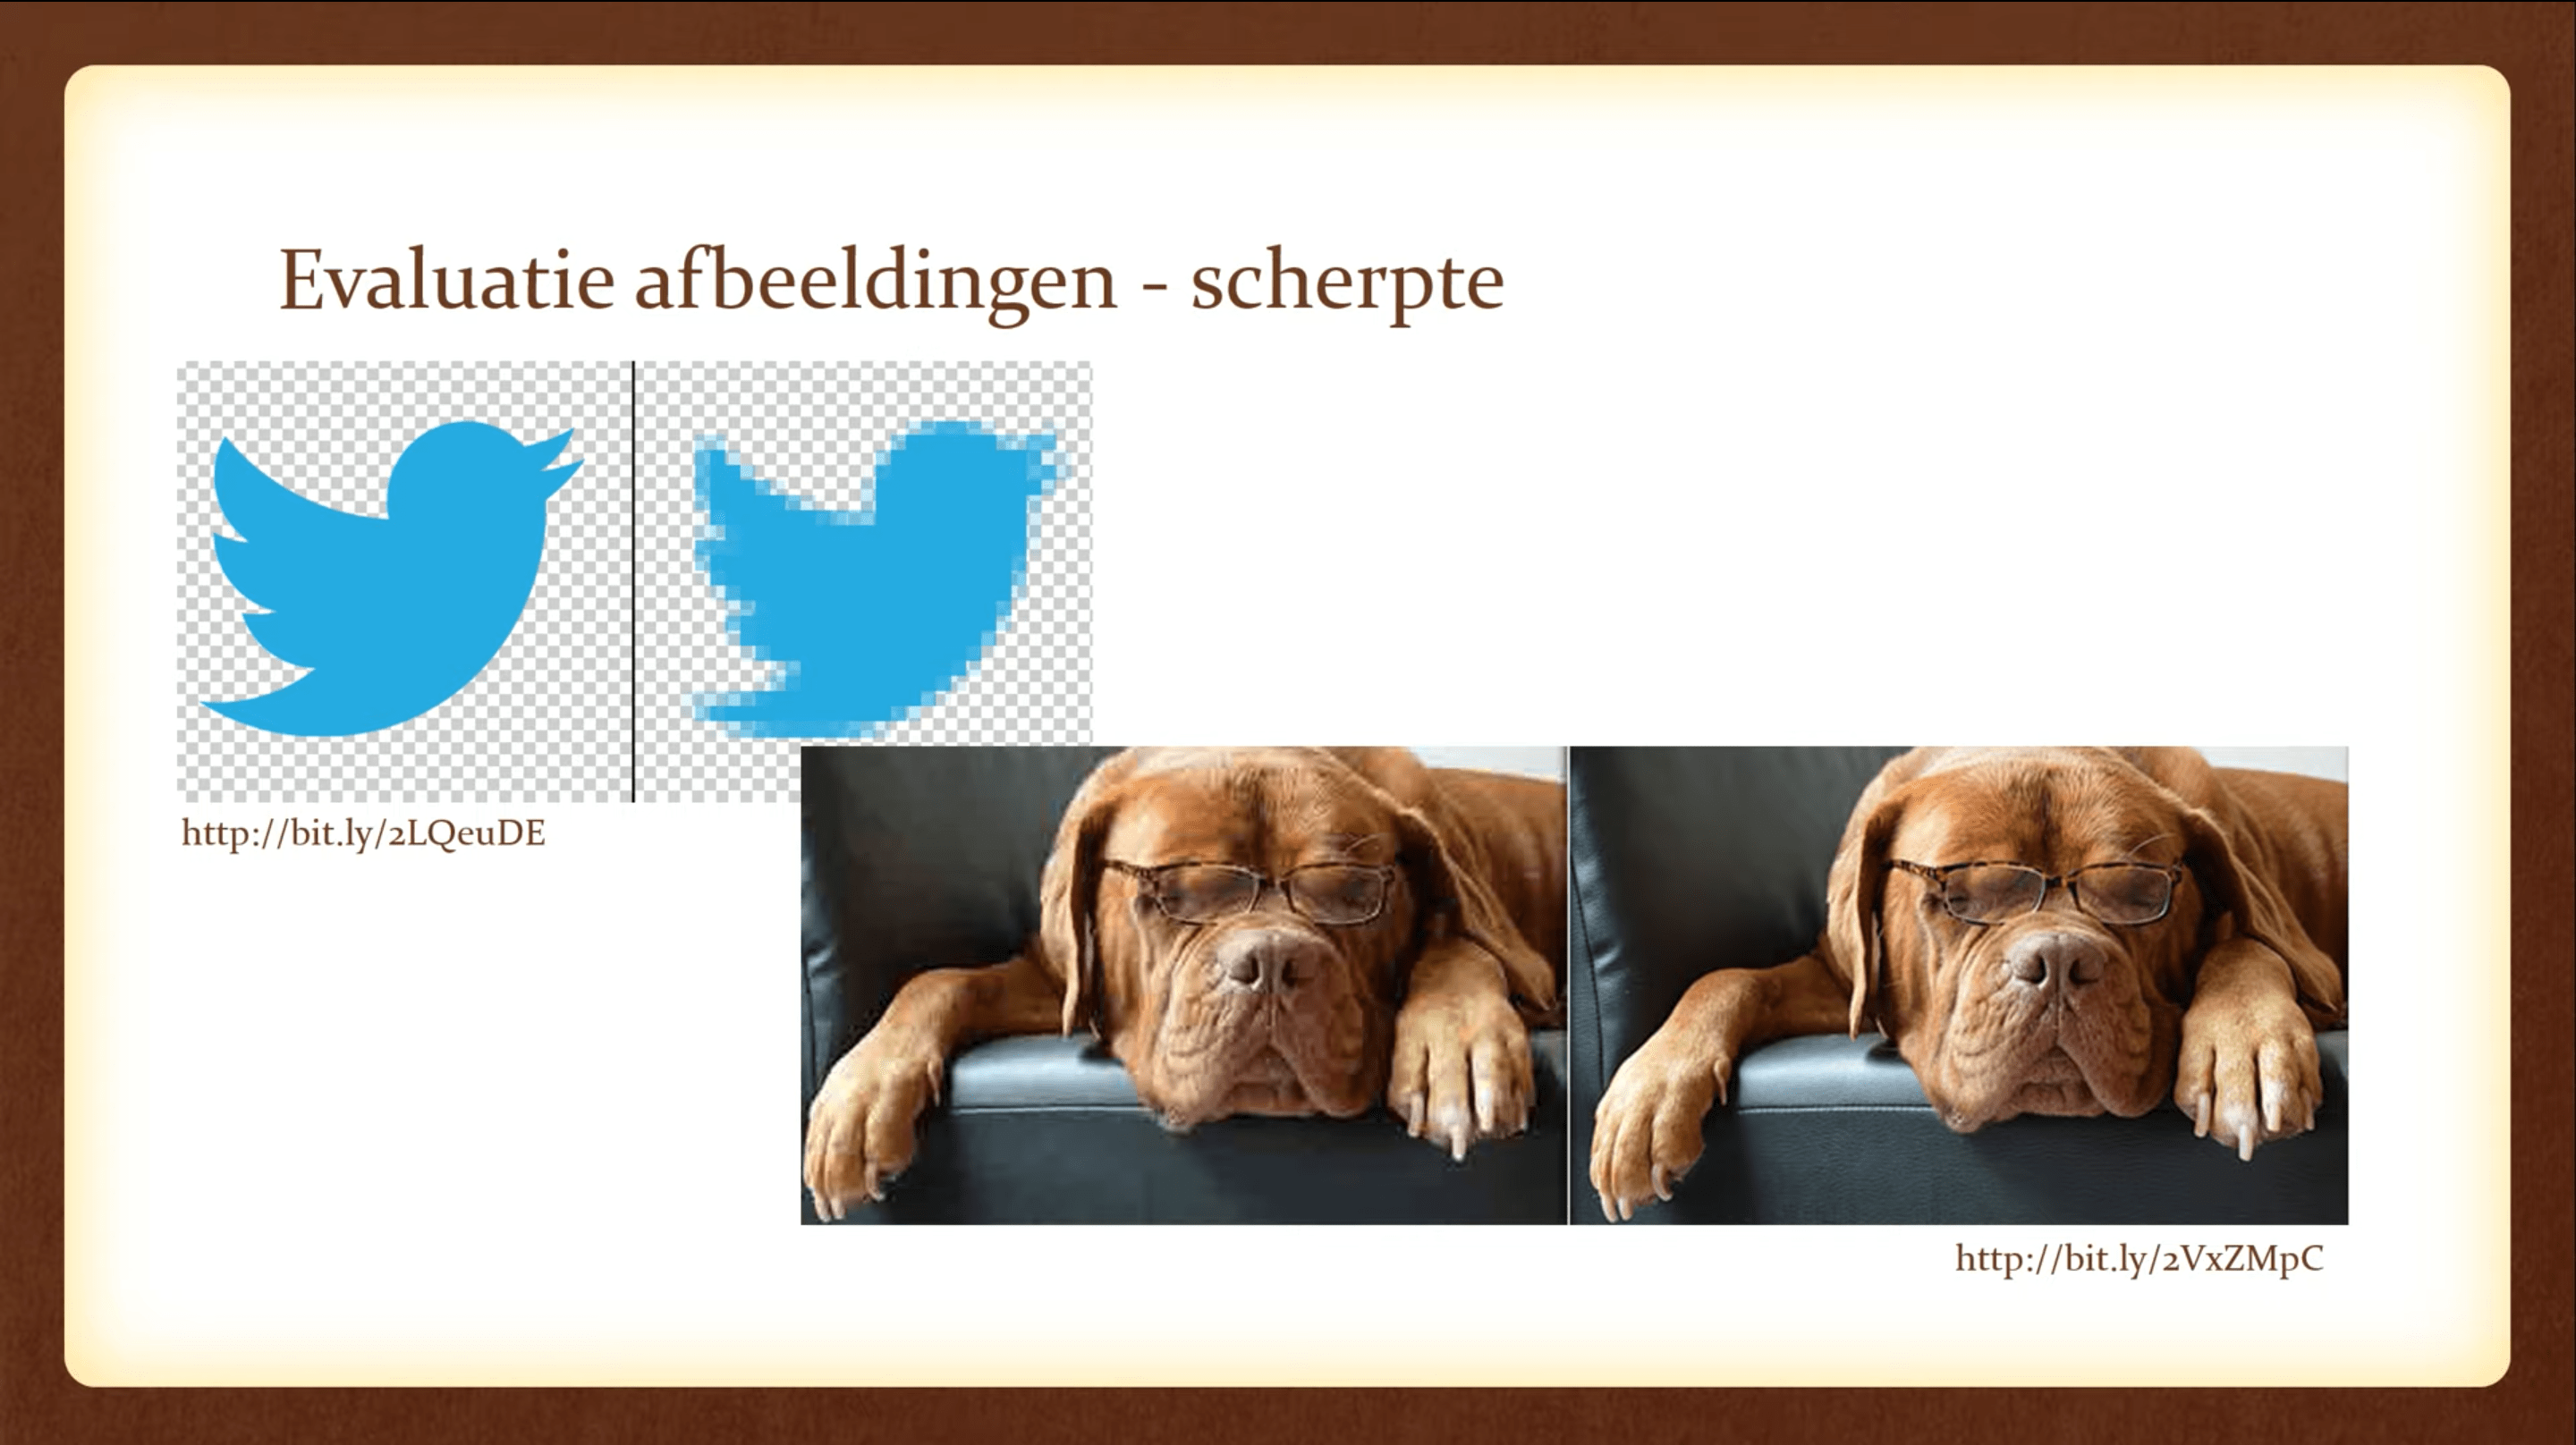
\includegraphics[width=\linewidth]{img/onderzoek/scherpte.png}
	\caption{Een fragment uit de introductievideo van de \gls{afbeeldingsevaluatietool} waarin het kenmerk scherpte (\ref{sec:onderzoek-evaluatietool-verloop-beoordeling-scherpte}) uitgelegd wordt. (\cite{introductievideo})}
	\label{fig:kenmerk-scherpte}
\end{figure}

\subsubsection{Kenmerk: kleuren en contrast}
\label{sec:onderzoek-evaluatietool-verloop-beoordeling-kleur}

Zoals hierboven besproken is de poot van de hond in figuur \ref{fig:kenmerk-scherpte} een goed voorbeeld van een slecht contrast. Op figuur \ref{fig:kenmerk-kleuren} is een fragment uit de introductievideo van de \gls{afbeeldingsevaluatietool} waarin het kenmerk kleur wordt uitgelegd zichtbaar. 

Hier worden vooral veelvoorkomende soorten \glspl{artefact} met betrekking op kleur weergeven. Bijvoorbeeld de \glspl{artefact} zichtbaar bij de ster door clustering in bijvoorbeeld het \gls{jpeg} \gls{afbeeldingsformaat}.

\FloatBarrier
\begin{figure}[h!]
	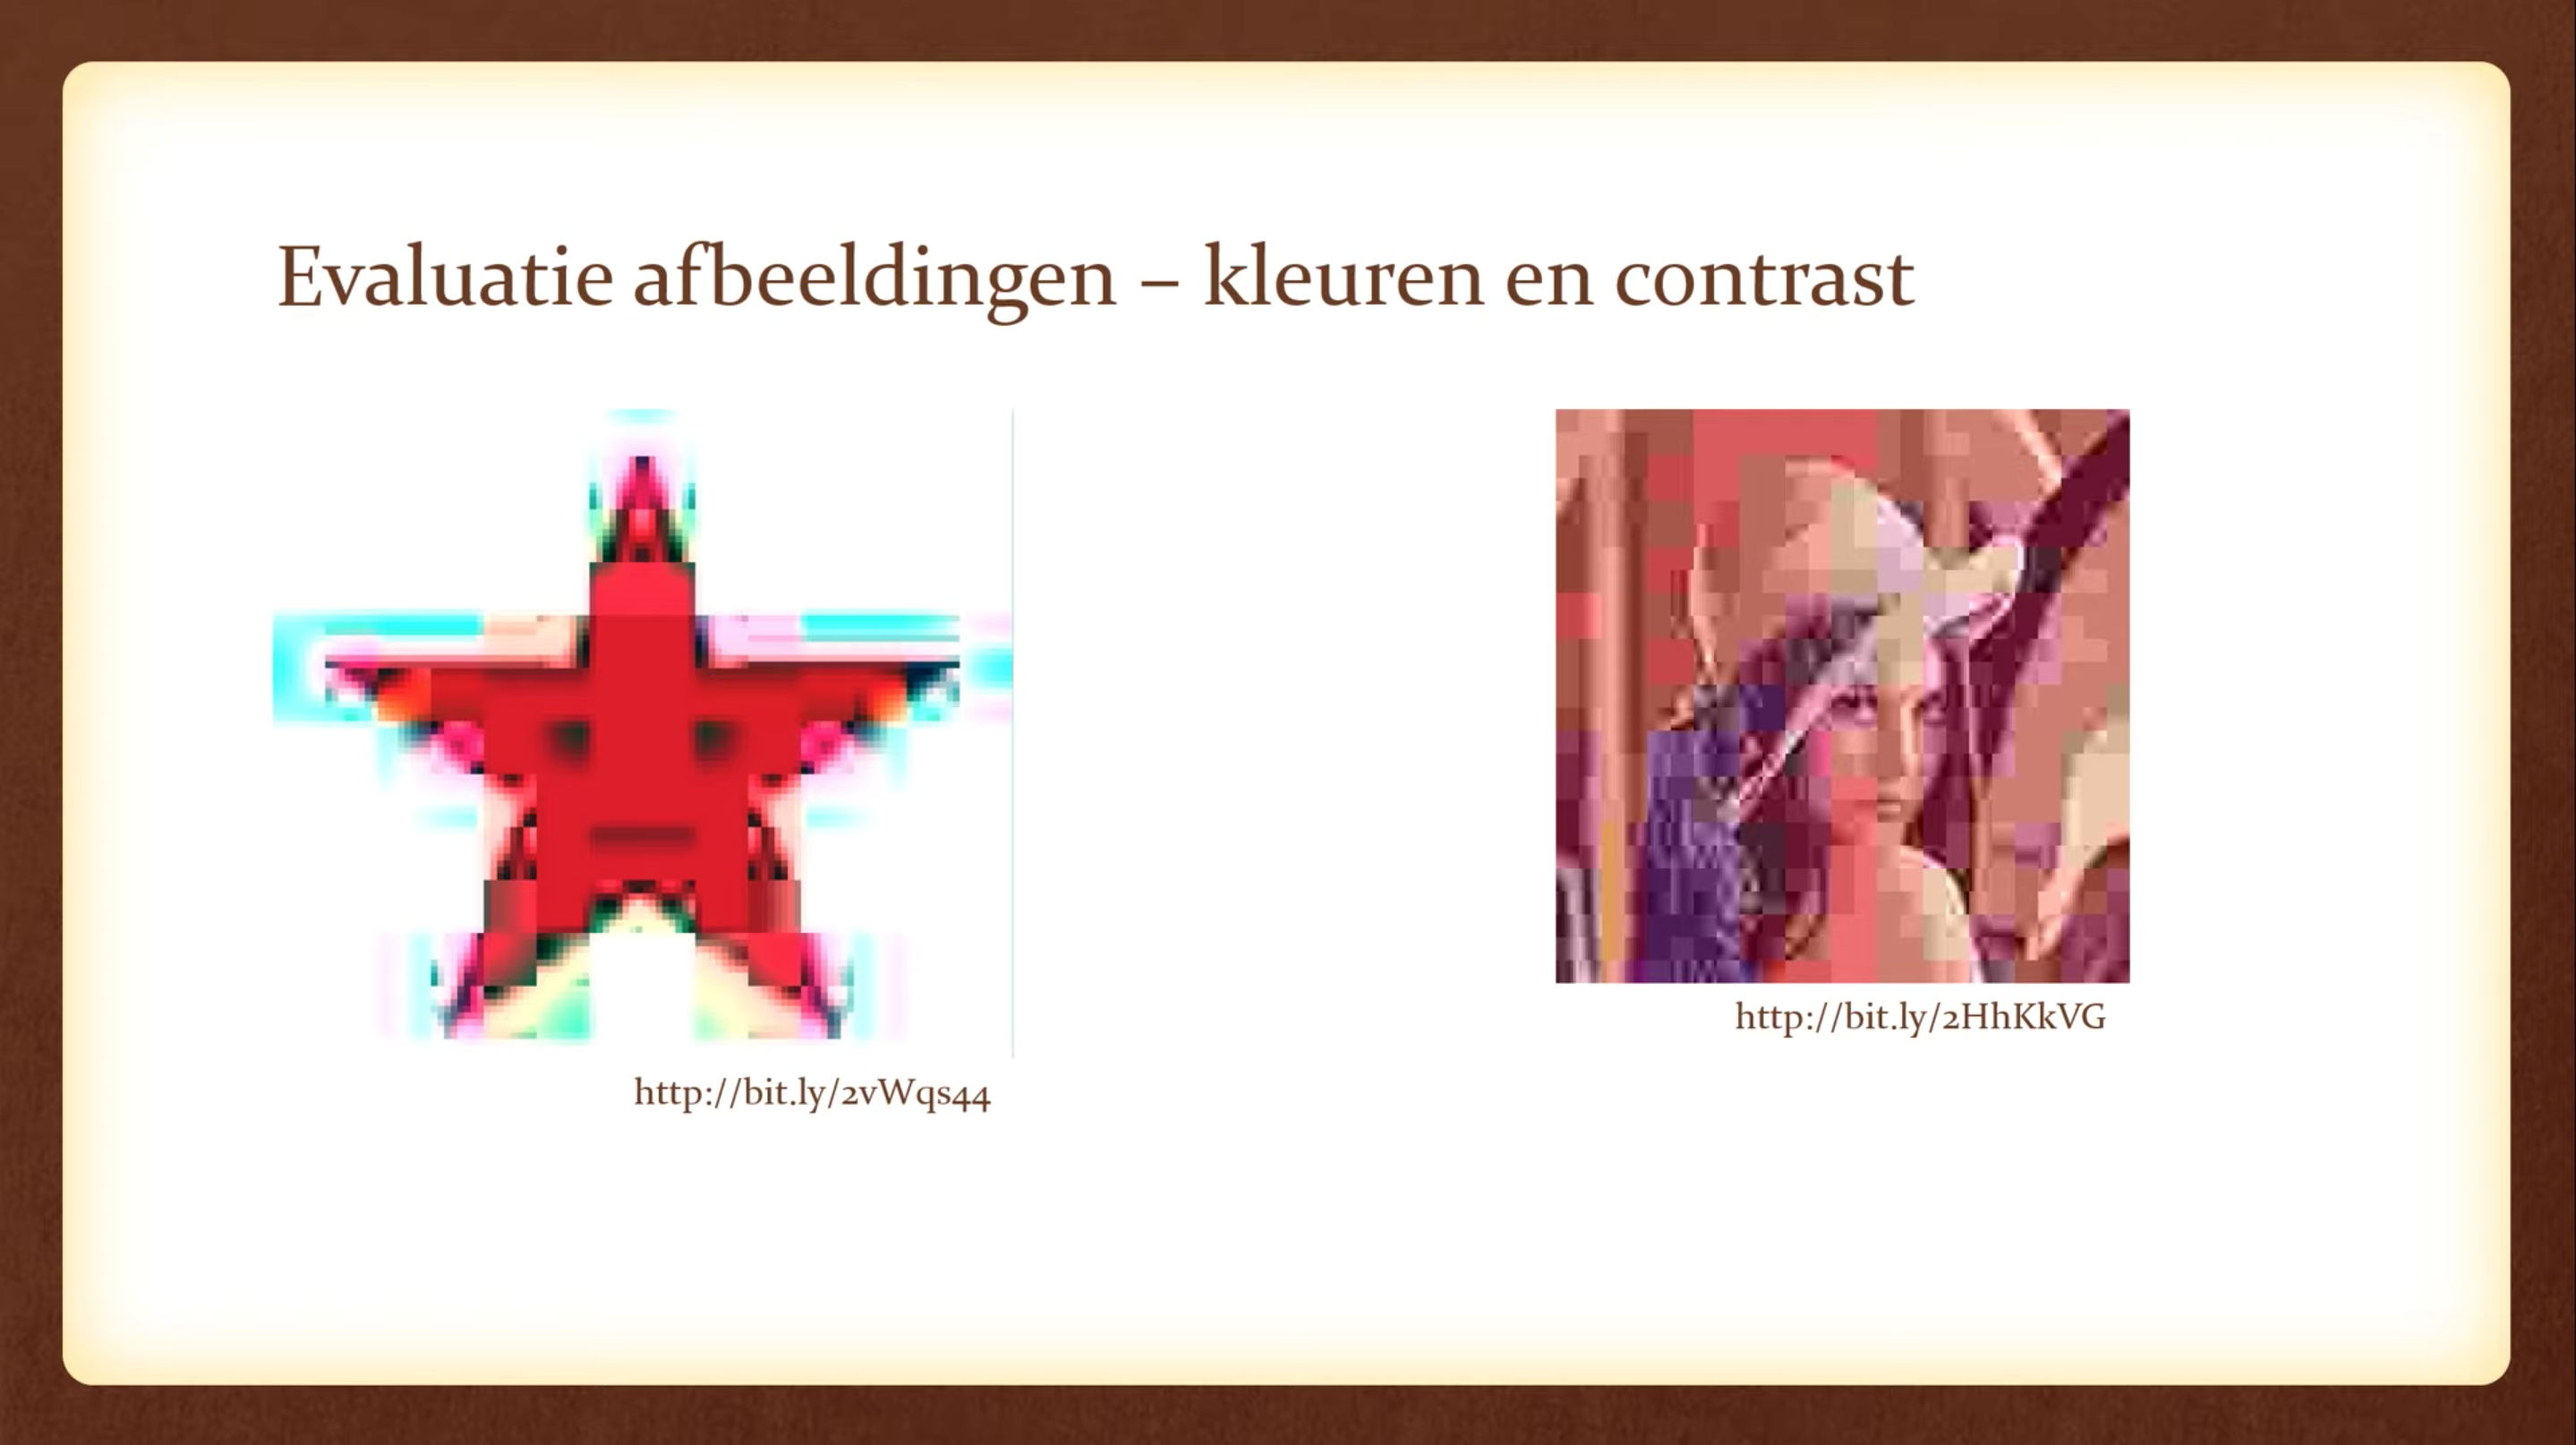
\includegraphics[width=\linewidth]{img/onderzoek/kleuren.png}
	\caption{Een fragment uit de introductievideo van de \gls{afbeeldingsevaluatietool} waarin het kenmerk kleuren en contrast (\ref{sec:onderzoek-evaluatietool-verloop-beoordeling-scherpte}) uitgelegd wordt. (\cite{introductievideo})}
	\label{fig:kenmerk-kleuren}
\end{figure}
\FloatBarrier

\subsubsection{Kenmerk: algemene indruk}
\label{sec:onderzoek-evaluatietool-verloop-beoordeling-algemeen}

Tot slot wordt ook de algemene indruk van de deelnemer gevraagd omtrent deze afbeelding. Hier is het belangrijk dat de score geven wordt vanuit het standpunt dat de foto is tegenkomen op de portfolio van een fotografe zoals meegeven in de \gls{use-case} (deel \ref{sec:onderzoek-use-case}).

\subsection{Exporteren van de verzamelde gegevens}
\label{sec:onderzoek-evaluatietool-export}

TODO
%TODO: onderzoek


\section{Uitvoering}
\label{sec:onderzoek-uitvoering}

TODO
%TODO: onderzoek

\subsection{Geëvalueerde afbeeldingsformaten}
\label{sec:onderzoek-uitvoering-afbeeldingsformaten}

TODO
%TODO: onderzoek

\subsection{Deelnemers}
\label{sec:onderzoek-uitvoering-deelnemers}

TODO
%TODO: onderzoek

\subsection{Opgeslagen data}
\label{sec:onderzoek-uitvoering-opgeslagen-data}

TODO
%TODO: onderzoek

\section{Resultaten}
\label{sec:onderzoek-resultaten}

TODO
%TODO: onderzoek

\section{Besluit}
\label{sec:onderzoek-besluit}

TODO
%TODO: onderzoek